\subsection{Schemat}
	\begin{center}
		\begin{figure}[h!]
			\makebox[\textwidth]{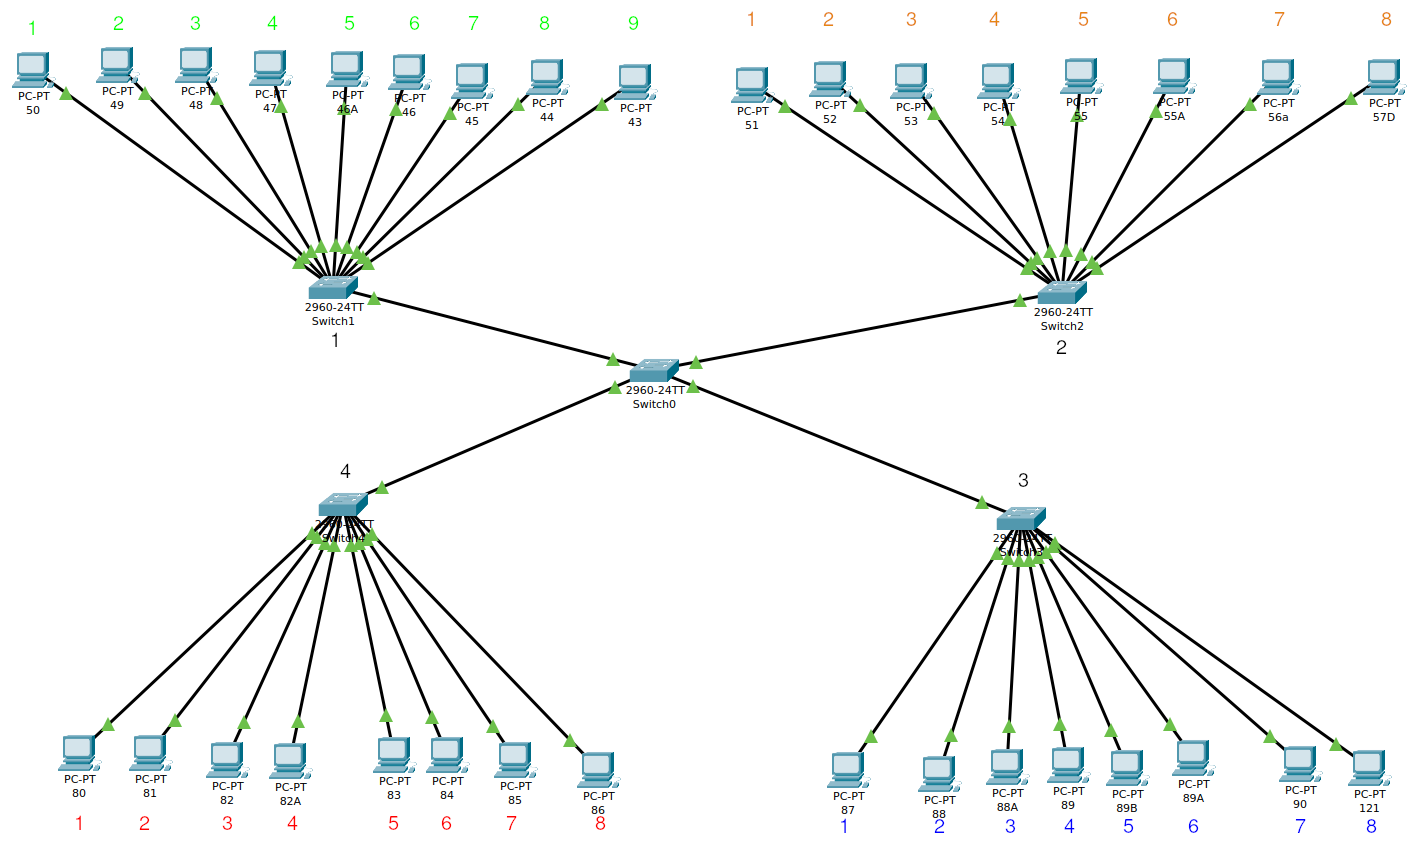
\includegraphics[width=\textwidth]{schemat_logiczny.png}}
			\caption{Schemat logiczny}
			\label{fig:schemat_logiczny}
		\end{figure}
		\begin{figure}[h!]
			\makebox[\textwidth]{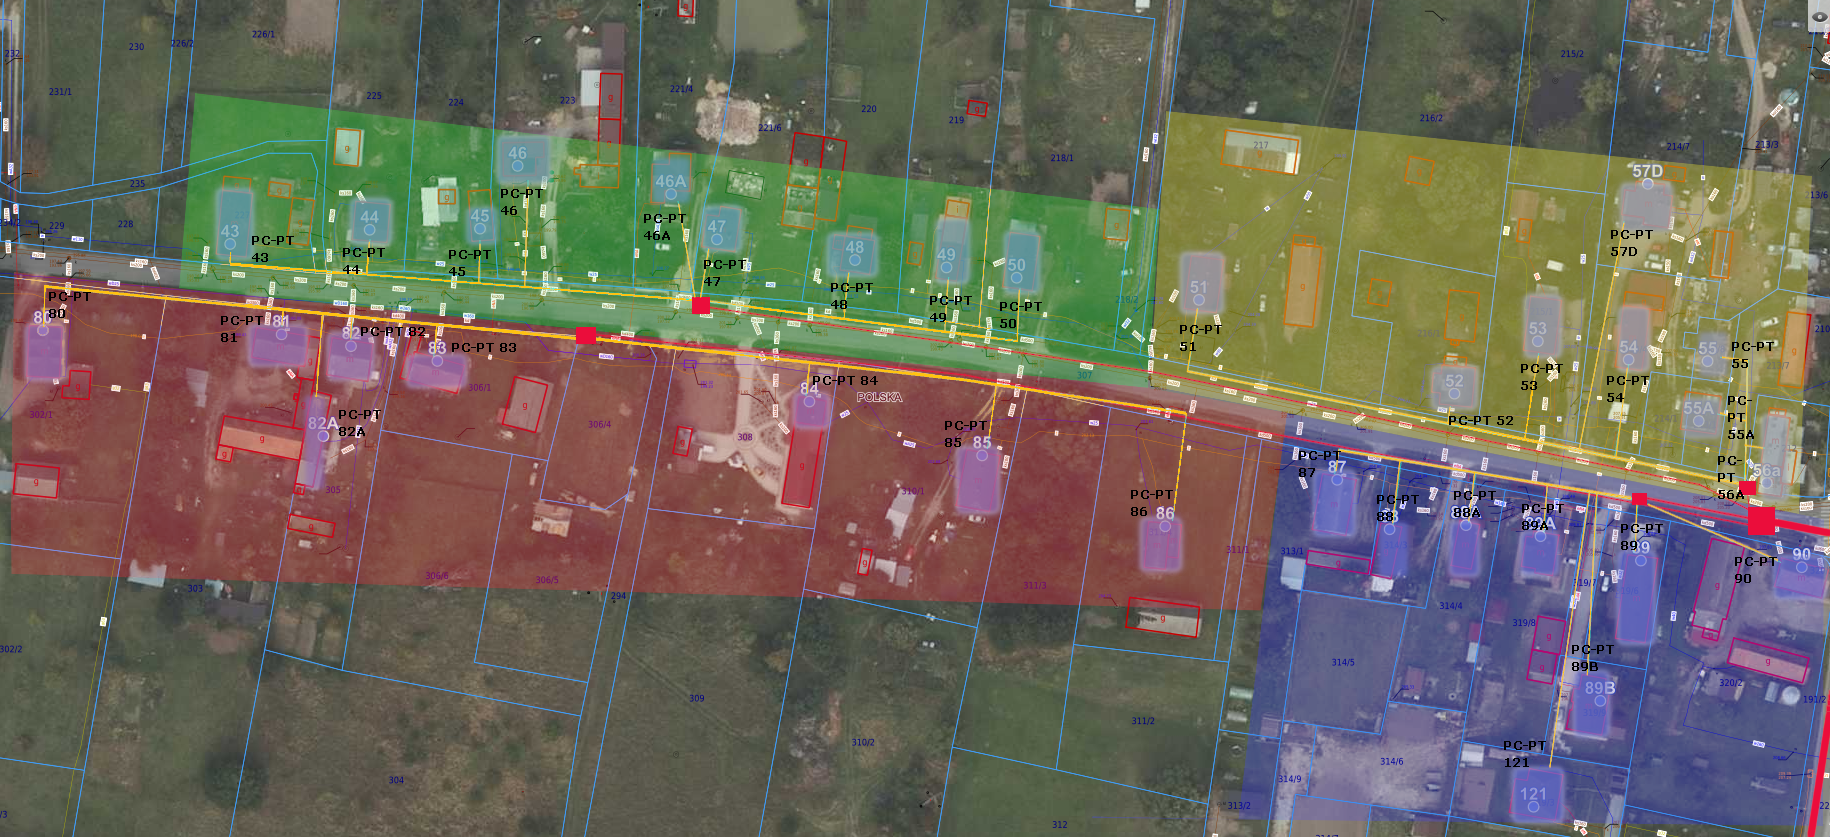
\includegraphics[width=\textwidth]{proj_gimp/proj.png}}
			\caption{Podział na podsieci na mapie fizycznej}
			\label{fig:podsieci}
		\end{figure}
	\end{center}

\subsection{Rozwiązania techologiczne}
	\paragraph{Okablowanie:}
		SM G657
	\paragraph{Złącza:}
		SC (Subscriber Connector)
	\paragraph{Użyte sprzęgacze:}
		\begin{center}
			\begin{table}[htbp]
				\begin{tabular}{|c|c|}
					\hline
					\textbf{Typ} & \textbf{ilość} \\ \hline
					1x4          & 1              \\ \hline
					1x16         & 4              \\ \hline
				\end{tabular}
			\end{table}
		\end{center}
	\paragraph{Porty:}
